\documentclass[preprint]{sigplanconf}

\usepackage{fixltx2e}

\usepackage[english]{babel}
\usepackage{amsmath,amssymb,array,listings}
\def\codefamily{\sffamily\normalsize}
\def\codesmall{\sffamily\small}

\usepackage{xspace}

\usepackage{todonotes}

\usepackage{framed}

\usepackage{xcolor}

\usepackage{tikz}
\usetikzlibrary{positioning,fit}
\usetikzlibrary{shapes.geometric}

\def\clash{C$\lambda$aSH\xspace}

\bibliographystyle{abbrvnat}

\begin{document}
\lstset{language=Haskell, basewidth=1.2ex, basicstyle=\codefamily, identifierstyle=\itshape,
 deletekeywords={String,Maybe,Just,Nothing,map,mapM,split,bracket,when,Bool,Int,div,round,sin,maxBound,fromIntegral,odd,True,False,Eq,negate,Double,Enum,index,fromEnum,not,accum,Functor,min,max,next,lookup,const,transpose,sum,sqrt,zipWith}} 

\title{Tranforming Programs into Application Specific Processors}
\authorinfo{Arjan~Boeijink \and Hendrik Folmer \and Jan~Kuper}{University of Twente}{\{w.a.boeijink,h.h.folmer,j.kuper\}@utwente.nl}

\maketitle

\begin{abstract}
The combination of performance and energy efficiency drives hardware designers to create specialized components for specific applications.
Current hardware technology has the space for complex algorithms to be mapped to hardware, however this complexity makes a manual hardware design process no longer tenable.
This paper shows that implementing a program as a specialised hardware design can be a systematic process using classic compiler techniques, and yields a processors-like architecture.
From programs written in an embedded Haskell DSL with explicit clock cycle boundaries we automatically generate a synthesizable hardware descriptions for application specific processors.
\end{abstract}


\section{Introduction}

Specialisation as key to hardware effiency. \\
FPGAs became large enough for many applications.
%FPGAs even available as accelerators for cloud computing.

%From the outside hardware is usually a small black box with number of pins connected to it.
%The inside a of chip consists of a large numbers of transistors are connected by wires.

% Some questions after reflecting on my own research:
\begin{itemize}
 \item What is the real difference between software and hardware?
 \item Why seems instruction set design obvious in hindsight?
 \item What are the important choices in ISA/processor design?
 \item How to make processor design a more systematic process?
\end{itemize}

Functional languages have a long history with hardware design \cite{Sheeran2005}

\subsection{Hardware in Haskell using \clash}
\clash \cite{Baaij} is a subset of Haskell that can be compiled to widely supported lower level hardware description languages such as Verilog and VHDL.
Even though you can use most abstractions that Haskell has to offer, \clash is still a structural hardware description language.

\subsection{The hardware design process in practice}
\begin{enumerate}
 \item Choose algorithm
 \item Convert math/pseudo code to executable Haskell
 \item fixed size vectors
 \item select numeric precision
 \item synthesize for hardware resource costs
 \item split algorithm in steps to reduce data access to feasible memory bandwith
 \item find patterns in algorithm to enable reuse of hardware components
 \item break long latency computation in parts to enable good clock frequencies
 \item write glue logic/control for pipelining and multistep computations
 \item synthesize design for target hardware platform
 \item iterate parts of this process until satisfied with performance/costs
\end{enumerate}
The nice aspect of this process is that every refinement of the design is described as executable haskell code.
Thus you can easily compare outputs of each step and see the impact of design choices on precission.
The downside is that you often come to conclusion that the algoritm choosen doesn't achieve the performance/costs you want. So you have to go through all steps again.
Steps 6 to 9 take the most effort, and step 9 is very error prone and can be very complex.

\section{Rewriting a program into a processor}
as a running example in this section we use a binary variant of greatest common divisor, that doesn't use any complex arithmetic operation:
\begin{lstlisting}
binGCD :: Word32 -> Word32 -> Word32       
binGCD x 0 = x
binGCD x y = let
    a = dropZeros x
    b = dropZeros y
    (s,g) = (min a b, max a b)
  in binGCD s (g - s) <<< countZeros (x .|. y)

dropZeros :: Word32 -> Word32
dropZeros i = i >>> countZeros i

countZeros :: Word32 -> Word32
countZeros n = if odd n then 0 
  else countZeros (n >>> 1) + 1
\end{lstlisting}
the count trailing zeros could been implemented as a primitive operation as a fold over bits

\subsection{Desugaring and flattening the program}
the first step is splitting up expressions which are too complex to execute within a single clock cycle \\
this can be done by introducing let expression like in the conversion to administrative normal form \cite{ANF} \\
the question is which expressions to define as trivial, for example some arithmetic operations mights be cheap enough to keep nested \\


\subsection{Making sequential execution explicit}
\begin{lstlisting}
binGCD x y k = if (y == 0)
  then cont x k
  else
    dropZeros x
      (\a -> dropZeros y
        (\b -> cont (max a b)
          (\g -> cont (min a b)
            (\s -> cont (g - s)
              (\d -> binGCD s d
                (\r -> cont (x .|. y)
                  (\o -> countZeros o
                    (\e -> cont (r <<< e) k)
      )))))))
\end{lstlisting}

translating recursive functions \cite{Ingmar} \cite{Zhai} \\
CPS transform \cite{AppelCwC} \\
defunctionalisation \cite{Reynolds} \\
combined in \cite{CCC}

\lstset{basicstyle=\codesmall}
\begin{lstlisting}
data Cont
  = CA Word32 Word32                      Cont
  | CB Word32 Word32 Word32               Cont
  | CC Word32 Word32 Word32 Word32        Cont
  | CD Word32 Word32 Word32 Word32 Word32 Cont

binGCD x y         k  = if (y == 0)
                   then cont x         k
                   else dropZeros x    (CA x y       k)
cont a (CA x y     k) = dropZeros y    (CB x y a     k)
cont b (CB x y a   k) = cont (max a b) (CC x y a b   k)
cont g (CC x y a b k) = cont (min a b) (CD x y a b g k)
\end{lstlisting}
\lstset{basicstyle=\codefamily}

\subsection{State machine with a stack}
combine functions into one by making each a data type, including the continuation application function \\
using the observation that nested continuations form a stack

\begin{lstlisting}
data Call = GCD Word32 Word32 | DropZs Word32
          | CntZs Word32 | Cont Word32
data Context
  = CA Word32 Word32
  | CB Word32 Word32 Word32
  | CC Word32 Word32 Word32 Word32
  | CD Word32 Word32 Word32 Word32 Word32
  ...
type Stack  = [Context]

step :: Call -> Stack -> (Call, Stack)
step (GCD x y)        cs = if y == 0
  then (Cont x      , cs               )
  else (DropZs x    , CA x y       : cs)
step (Cont a)        (CA x y       : cs) =
     (DropZs y      , CB x y a     : cs)
step (Cont b)        (CB x y a     : cs) =
     (Cont (max a b), CC x y a b   : cs)
step (Cont g)        (CC x y a b   : cs) =
     (Cont (min a b), CD x y a b g : cs)
\end{lstlisting}

\begin{figure}
\centering
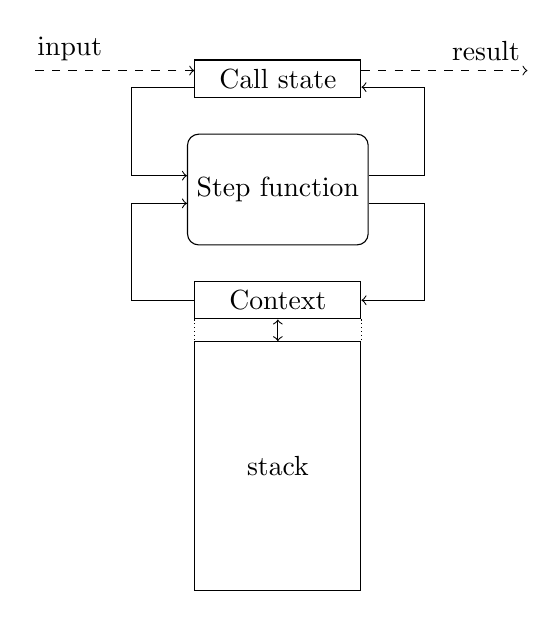
\begin{tikzpicture}
\node[draw, shape=rectangle, minimum width=6em] (st) {Call state};
\node[draw, shape=rectangle, minimum width=6em, minimum height=4em, below of=st, node distance=4em, rounded corners] (fun) {Step function};
\node[draw, shape=rectangle, minimum width=6em, below of=fun, node distance=4em] (con) {Context};
\node[draw, shape=rectangle, minimum width=6em, minimum height=9em, below of=con, node distance=6em] (ck) {stack};
\draw[densely dotted] (con.south west) -- (ck.north west);
\draw[densely dotted] (con.south east) -- (ck.north east);
\draw[->, dashed] ([yshift=0.3em]st.east) -- node[above, near end] {result} ([yshift=0.3em,xshift=6em]st.east);
\draw[<-, dashed] ([yshift=0.3em]st.west) -- node[above, near end] {input} ([yshift=0.3em,xshift=-6em]st.west);
\draw[->] ([yshift=0.5em]fun.east) -| ([xshift=2em]fun.north east) |- ([yshift=-0.3em]st.east);
\draw[->] ([yshift=-0.3em]st.west) -| ([xshift=-2em]fun.north west) |- ([yshift=0.5em]fun.west);
\draw[->] ([yshift=-0.5em]fun.east) -| ([xshift=2em]fun.south east) |- (con.east);
\draw[->] (con.west) -| ([xshift=-2em]fun.south west) |- ([yshift=-0.5em]fun.west);
\draw[<->] (con.south) -- (ck.north);
\end{tikzpicture}
\caption{Hardware structure of the stack machine}
\end{figure}

\subsection{Separating the data stack}

lots of data copied from one state/continuation to another \\
and stack is very wide because some continuations capture a lot of free variables \\
only a few are used/produced every cycle \\
note that we have to copy the argument to the dropZeros function because they are used again and/or in the wrong order \\
for the arguments to the recursive binGCD call we can skip copying as they are in the right order and not used later

\begin{lstlisting}
data State = BinGCD | DropZs | CntZs | Cont
data Context = CA | CB | CC | CD | ...
type CtrlStack  = [Context]
type DataStack = [Word32]

step ::  State -> CtrlStack -> DataStack ->
  (State, CtrlStack, DataStack)
step BinGCD     cs      (y:x:ds) = if y == 0
  then (Cont  , cs   ,     x:ds)
  else (DropZs, CA:cs, x:y:x:ds)
step Cont (CA:cs)     (a:y:x:ds) = 
  (DropZs, CB:cs,    y:a:y:x:ds)
step Cont (CB:cs)   (b:a:y:x:ds) = 
  (Cont,   CC:cs,  g:b:a:y:x:ds) where g = max a b
step Cont (CC:cs) (g:b:a:y:x:ds) = 
  (Cont,  CD:cs, s:g:b:a:y:x:ds) where s = min a b
\end{lstlisting}

having two stacks might look like a unnecessary complication from the C-like software stack point of view, but is common in hardware designs based on Forth \cite{LaForest}

\subsection{Optimizing control}

What happens in every step can depend on both the state and top of the continuation stack. \\
combine state and continuation stack in a control stack by eliminating the Return state. \\
now only the top of the control stack directly determines what each step does. \\
the top of the control stack is effectively a program counter \\
a program counter is merely a numeric encoded label optimized for the common case of continuing at the successive label \\
the steps with if expressions are more complex than the rest, and can be split up by computing the branch condition in a separate step

\begin{lstlisting}
data Label = BinGCD | T1 | E1 | CA | CB | CC
   | CDE | DropZs | ... deriving Enum
type ControlStack  = [Label]
type DataStack = [Word32]
type CtrlFun = Label -> CtrlStack -> 
  (Label, CtrlStack)

step :: Label -> DataStack -> (CtrlFun,DataStack)
step BinGCD        (y:x:ds) =
  (branch E1 z,     y:x:ds) where z = y == 0
step T1            (y:x:ds) = 
  (ret        ,       x:ds)
step E1            (y:x:ds) = 
  (call DropZs,   x:y:x:ds)
step CA          (a:y:x:ds) = 
  (call DropZs, y:a:y:x:ds)
step CB        (b:a:y:x:ds) = 
  (next     , g:b:a:y:x:ds) where g = max a b
step CC      (g:b:a:y:x:ds) = 
  (next   , s:g:b:a:y:x:ds) where s = min a b
\end{lstlisting}

the resulting dual stack machine looks like something you could derive by looking at the flattened program from tradition imperative language point of view

\subsection{Splitting into components}

to use efficient existing memory components we have to split each step in parts to seperate memory read and write actions \\
also splitting off the arithmetic operations makes it easier to reuse hardware for similiar computations

\begin{lstlisting}
type CtrlFun = Word32 -> Label -> CtrlStack ->
   (Label, CtrlStack)
type Input = DataStack -> Word32
type AluOp = Word32 -> Word32 -> Word32
type StackMod = Word32 -> DataStack -> DataStack
\end{lstlisting}

\lstset{basicstyle=\codesmall}
\begin{lstlisting}
step :: Label -> (CtrlFun,Input,Input,AluOp,StackMod)
step GCD = (branch E1  ,peek 0,lit 0 , isEq ,keep)
step T1  = (ret        ,peek 1,lit 0 , pass ,popNPush 2)
step E1  = (call DropZs,peek 1,lit 0 , pass ,push)
step CA  = (call DropZs,peek 1,lit 0 , pass ,push)
step CB  = (next       ,peek 1,peek 0, max  ,push)
step CC  = (next       ,peek 2,peek 1, min  ,push)
\end{lstlisting}
\lstset{basicstyle=\codefamily}

\subsection{Control by microcode}

each step now produces a set of functions, however functions can not directly exist in hardware \\
thus we apply defunctionalisation to each component \\
the resulting structure is like a processor controlled by horizontal microcode

\begin{lstlisting}
data AluOp = Const | Add | Sub | Or | Min | Max |
   ShR | ShL | IsEq | IsOdd
data Input = S Int | I Word32
data StAction = Keep | Push | PopNPush Int
data Ctrl = Call Label |Return |Branch Label |Next
\end{lstlisting}

\lstset{basicstyle=\codesmall}
\begin{lstlisting}
microcode :: Label -> (Ctrl,Input,Input,AluOp,StAction)
microcode pc = case pc of
  BinGCD -> (Branch E1  , S 0, I 0, IsEq , Keep)
  T1     -> (Return     , S 1, I 0, Pass , PopNPush 2)
  E1     -> (Call DropZs, S 1, I 0, Pass , Push)
  CA     -> (Call DropZs, S 1, I 0, Pass , Push)
  CB     -> (Next       , S 1, S 0, Max  , Push)
  CC     -> (Next       , S 2, S 1, Min  , Push)
  CDE    -> (Call BinGCD, S 1, S 0, Sub  , Push)
  CFG    -> (Call CntZs , S 5, S 4, Or   , Push)
  CH     -> (Return     , S 1, S 0, ShL  , PopNPush 7)
  DropZs -> (Call CntZs , S 0, I 0, Pass , Push)
  CI     -> (Return     , S 1, S 0, ShR  , PopNPush 2)
  CntZs  -> (Branch E2  , S 0, I 0, IsOdd, Keep)
  T2     -> (Return     , I 0, I 0, Pass , PopNPush 1)
  E2     -> (Call CntZs , S 0, I 1, ShR  , Push)
  CK     -> (Return     , S 0, I 1, Add  , PopNPush 2)
\end{lstlisting}
\lstset{basicstyle=\codefamily}

\begin{lstlisting}
alu :: AluOp -> Word32 -> Word32 -> Word32
alu Pass  x _ = x
alu Add   x y = x + y
alu Sub   x y = x - y
alu Or    x y = x .|. y
alu Min   x y = min x y
alu Max   x y = max x y
alu ShR   x y = x >>> y
alu ShL   x y = x <<< y
alu IsEq  x y = if x == y then 1 else 0
alu IsOdd x _ = if odd x then 1 else 0

selInput :: DataStack -> Input -> Word32
selInput ds (S i) = ds !! i
selInput _  (I x) = x

stackMod :: StAction -> Word32 -> 
  DataStack -> DataStack
stackMod Keep             = keep
stackMod Push             = push
stackMod (PushAfterPop n) = pushAfterPop n

ctrl :: Ctrl -> Word32 -> Label -> [Label] ->
  (Label, [Label])
ctrl Next       = next
ctrl Return     = ret
ctrl (Branch e) = branch e
ctrl (Call f  ) = call f
\end{lstlisting}

\subsection{Synthesisable implementation in \clash}
the main effort of converting into a synthesisable hardware description is replacing the lists for the control and data stack with memory components and stack pointers \\
both stackpointer and the program counter need to be saved in a register \\
the $microcode$ and $alu$ code from previous step can be directly reused with any change \\
all components are then connected together in the toplevel of the processor description \\
this is straightforward except for having to work with Signal's instead of pure values

\begin{lstlisting}
proccesor :: Signal () -> Signal (Label, Word32)
proccesor _ = bundle (pc, z) where
  pc = register def pc'
  (ctrlOp,ia,ib,oper,stOp) = liftB microcode pc

  nPC = liftA succ pc
  (cSP', savePC, pc') = 
    liftB5 ctrl ctrlOp z nPC cSP retPC
  cSP = register 0 cSP'
  retPC = asyncRam d64 cSP savePC

  rdA = liftA2 agu dSP ia
  rdB = liftA2 agu dSP ib
  a = asyncRam d128 rdA wrData
  b = asyncRam d128 rdB wrData

  x = liftA2 inputMux ia a
  y = liftA2 inputMux ib b
  z = liftA3 alu oper x y

  dSP = register 0 dSP'
  (dSP', wrData) = liftB3 stackMod stOp dSP z
\end{lstlisting}

\begin{lstlisting}
agu :: Word8 -> Input -> Word8
agu stackSp (S i) = stackSp - i
agu stackSp (I _) = stackSp

ctrl :: Ctrl -> Word32 -> Label -> Word8 -> Label
  -> (Word8, Maybe (Word8, Label), Label)
ctrl Next       _ nPC cSP retPC =
  (cSP  , Nothing          , nPC)
ctrl Return     _ nPC cSP retPC =
  (cSP-1, Nothing          , retPC)
ctrl (Branch e) 0 nPC cSP retPC =
 (cSP  , Nothing          , e)
ctrl (Branch e) _ nPC cSP retPC =
  (cSP  , Nothing          , nPC)
ctrl (Call f)   _ nPC cSP retPC =
  (cSP+1, Just (cSP+1, nPC), f)

stackMod :: StAction -> Word8 -> Word32 ->
  (Word8, Maybe (Word8, Word32))
stackMod Keep         dSP z =
  (dSP , Nothing)
stackMod Push         dSP z =
  (dSP', Just (dSP', z)) where dSP' = dSP+1
stackMod (PopNPush n) dSP z =
  (dSP', Just (dSP', z)) where dSP' = dSP-n+1
\end{lstlisting}


\subsection{The derived hardware architecture}
\begin{figure}
\centering
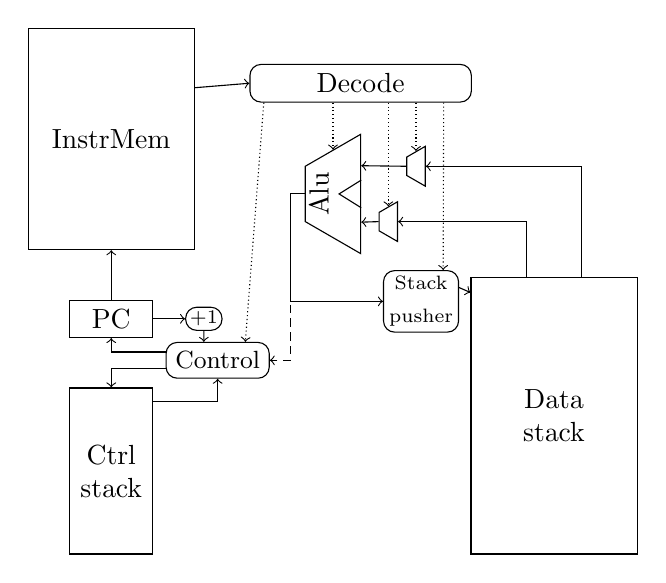
\begin{tikzpicture}
\node[draw, shape=rectangle, minimum width=6em, minimum height=8em] (im) {InstrMem};
\node[draw, shape=rectangle, rounded corners, minimum width=8em, above right of=im, xshift=7em] (dec) {Decode};
\node[draw, shape=rectangle, minimum width=3em, below of=im, node distance=6.5em] (pc) {PC};
\node[draw, shape=rectangle, rounded corners, right of=pc, xshift=0.5em, inner sep=0.15em] (npc) {\begin{scriptsize}$+1$\end{scriptsize}};
\node[draw, shape=rectangle, rounded corners, right of=pc, xshift=1em, yshift=-1.5em] (cc) {\begin{small}Control\end{small}};
\node[draw, shape=rectangle, minimum width=3em, minimum height=6em, below of=pc, node distance=5.5em, align=center] (cs) {Ctrl\\stack};
\node[draw, shape=rectangle, minimum width=6em, minimum height=10em, below of=im, node distance=10em, align=center, xshift=16em] (ds) {Data\\stack};
\node[draw, shape=trapezium, minimum width=3em, minimum height=2em, below of=dec, node distance=4em, xshift=-1em, rotate=90] (alu) {};
\node[xshift=-0.5em, rotate=90] at (alu.center) {Alu};
\node[draw, shape=rectangle, rounded corners, below right of=alu, node distance=4.5em, yshift=-0.7em, inner sep=0.2em, align=center] (sp) {\begin{scriptsize}Stack\end{scriptsize}\\\begin{scriptsize}pusher\end{scriptsize}};
\draw ([yshift=0.5em] alu.south) -- ([xshift=-0.8em] alu.south) -- ([yshift=-0.5em] alu.south);
\node[draw, shape=trapezium, minimum width=1em, minimum height=0.5em, right of=alu, node distance=3em, yshift=1em, rotate=90] (ina) {};
\node[draw, shape=trapezium, minimum width=1em, minimum height=0.5em, right of=alu, node distance=2em, yshift=-1em, rotate=90] (inb) {};
\draw[->] (ina.north) -- (alu.south east);
\draw[->] (inb.north) -- (alu.south west);
\draw[->] ([xshift=1em] ds.north) |- (ina.south);
\draw[->] ([xshift=-1em] ds.north) |- (inb.south);
\draw[->] (pc.north) -- (im.south);
\draw[->] (pc.east) -- (npc.west);
\draw[->] (npc.south) -- ([xshift=-0.5em] cc.north);
\draw[->] ([yshift=1.85em] im.east) -- (dec.west);
\draw[->] ([yshift=0.3em] cc.west) -| (pc.south);
\draw[->] ([yshift=-0.3em] cc.west) -| (cs.north);
\draw[->] ([yshift=2.5em]cs.east) -| (cc.south);
\draw[->] ([yshift=0.5em] sp.east) -- ([yshift=4.45em] ds.west);
\draw[->] (alu.north) -- ([xshift=-0.5em] alu.north) |- (sp.west);
\draw[->, densely dashed] (alu.north) -- ([xshift=-0.5em] alu.north) |- (cc.east);
\draw[->, densely dotted] ([xshift=-3.5em] dec.south) -- ([xshift=1em] cc.north);
\draw[->, densely dotted] ([xshift=-1em] dec.south) -- (alu.east);
\draw[->, densely dotted] ([xshift=1em] dec.south) -- (inb.east);
\draw[->, densely dotted] ([xshift=2em] dec.south) -- (ina.east);
\draw[->, densely dotted] ([xshift=3em] dec.south) -- ([xshift=0.8em]sp.north);
\end{tikzpicture}
\caption{Architecture of derived processor}
\end{figure}

\subsection{Differences with common processors}

The downside of using horizontal microcode is that it costs a lot of bits to encode each step in the program \\
also writing microcode by hand is a lot of work \\
thus almost all processors define an instruction set that provides a slightly higher way of writing programs \\
from the processor point of view an instruction set is just a compressed form of microcode with a hardware component for decoding (decompressing) \\
secondly an instruction set gives the oppertunity of improving the next generation of a processor design without having to change all software

\begin{lstlisting}
instrMem :: [(Label, Instr)]
decode :: Instr->(Input,Input,Oper,StAction,Ctrl)

selInput :: DataStack -> Input -> Word32
alu :: Oper -> Word32 -> Word32 -> Word32
stackMod :: StAction->Word32->DataStack->DataStack
ctrl :: Ctrl -> Word32 -> CtrlStack -> CtrlStack

sim :: DataStack -> [Label] -> Word32
sim ds []       = top ds
sim ds (pc:cs) = sim ds' cs' where
  Just is = P.lookup pc instrMem
  (ia, ib, op, g, f) = decode is
  x = selInput ds ia
  y = selInput ds ib
  z = alu op x y 
  ds' = stackMod g z ds
  cs' = ctrl f z (pc : cs)

\end{lstlisting}

heap memory \\
input/ouput 

\section{A DSL for explicitly clocked programs}
When designing application specific hardware components we care a lot about performance and/or efficiency, otherwise we could have used some existing processor.
The gains come from doing some specialised computation in less steps (clock cycles) and/or doing more operations in parallel than a normal processor could.
While the transformation process described in previous produces a working processor, it is fairly minimalistic and not that efficient.
The decision of how much computation to do in each step is a complex optimisation problem that depends on area and clock frequency requirements.
Thus we leave it up to the hardware designer to explicitly decide how to group computations into clock cycles.
Also the timing with respect to other components can be important, so the order of execution of each cycle needs to be explicit.

\subsection{More control over memory}
explicit allocation of writable memory addresses\\
indexing in larger memory structures

\subsection{Existing components as coprocessors}
Complex arithmetic operations such as divisions, square root and trigonometric functions are usually implemented as seperate components that take many cycles to execute. \\
a coprocessor can be described as just function in the same EDSL \\
the coprocessor executes concurrently after forking it from main program, and you can wait for its finished results by joining it

\subsection{Vectorisation support}
One of the most important ways to achieve higher performance in specialized hardware is to do a lot things in parallel.
However the amount of available parallism is often larger than what fits on the limited area of the hardware.
Thus we have split operations on large vectors into segments which are executed over time. \\

\textit{Work in progress, to be extended}


\subsection{Software pipelining}
Dependencies between operations can lead to poor utilisation of the available hardware resources.\\
If long dependencies chains exist within a loop, the performance might be improved by (partial) overlapping of the execution of multiple loop iterations. \\
This technique is known as software pipeling and is commonly used in compilers for VLIW processors.

\subsection{Cycle accurate simulation}
programs are usually part of a larger system \\
for cosimulation with other component written in \clash we support running a $Seqlogic$ program as a signal function \\
this allows whole system simulation and analysis in early stages of the design process
\begin{lstlisting}
interpretSeqLogic :: (forall s. SeqLogic s i o ())
  -> Signal (Maybe i) -> Signal (Maybe o)
\end{lstlisting}
this cycle by cycle simulation is implemented using the operational monad technique, where $clock$ statements suspend the computation \\
memory is implemented using the lazy ST monad \\
for coprocessors a list of active ones is maintained and each one is run at every $clock$ statement in the main program



\section{Example application: ICP}
iterative closest point is an algorithm used for position finding using a laser range finder \cite{Robin:Hendrik}

\lstset{basicstyle=\codesmall}

\begin{lstlisting}
qr :: SeqLogic s [Double] [[Double]] ()
qr = do
   v0 <- receive
   clock
   v1 <- receive
   clock
   v2 <- receive
   clock
   v3 <- receive
   clock
   
   let y0 = v0
   u0 <- call $ norm y0

   v1_u0 <- call $ v1 `dotp_scale` u0
   clock
   let y1 = v1 .-. v1_u0
   
   u1 <- call $ norm y1

   v2_u0 <- call $ v2 `dotp_scale` u0

   v2_u1 <- call $ v2 `dotp_scale` u1
   clock
   let sa = v2 .-. v2_u0
   clock
   let y2 = sa .-. v2_u1

   u2 <- call $ norm y2

   v3_u0 <- call $ v3 `dotp_scale` u0

   v3_u1 <- call $ v3 `dotp_scale` u1

   v3_u2 <- call $ v3 `dotp_scale` u2
   clock
   let sb = v3 .-. v3_u0
   clock
   let sc = sb .-. v3_u1
   clock
   let y3 = sc .-. v3_u2

   u3 <- call $ norm y3
   clock
   
   let q' = [u0, u1, u2, u3]

   let a = transpose [v0,v1,v2,v3]
   
   r <- call $ mat_mul q' a
   clock
   emit (transpose r)
\end{lstlisting}


\begin{lstlisting}
norm :: [Double] -> SeqLogic s i o [Double]
norm xs = do
   let sqs = xs .*. xs
   clock
   let n = sum sqs
   clock
   let invsq = 1/(sqrt n)
   clock
   return (invsq *. xs)

dotp_scale::[Double]->[Double]->SeqLogic s i o [Double]
dotp_scale vs us = do
   let zs = vs .*. us
   clock
   let n = sum zs
   clock
   return (n *. us)
\end{lstlisting}


\begin{lstlisting}
-- matrix multiplication using one dot product at a time
mat_mul :: [[Double]]->[[Double]]->SeqLogic s i o [[Double]]
mat_mul m1 m2 = do
   let m2' = transpose m2
   call $ seqMap (row_mul m1) m2'

row_mul m1 v = seqMap (dotp v) m1

dotp :: [Double] -> [Double] -> SeqLogic s i o Double
dotp xs ys = do
   let zs = xs .*. ys
   clock
   return (sum zs)

-- sequentially mapping over a list using an extra cycle for each element
seqMap :: (a->SeqLogic s i o b)->[a]->SeqLogic s i o [b]
seqMap f [] = return []
seqMap f (x:xs) = do
   y <- f x
   ys <- call $ seqMap f xs
   return (y:ys)

n *. xs = map (n*) xs
(.*.) = zipWith (*)
(.+.) = zipWith (+)
(.-.) = zipWith (-)
\end{lstlisting}

\lstset{basicstyle=\codefamily}

\subsection{Comparison with manual designed hardware}
compare hendrik implementation with the generated results from this section \\
apply high level optimizations beyond above designs

\subsection{Optimizing the ICP implementation}
software pipelining the nearest 2 points loop \\
alu output register and computation reordering to use only single memory read port

\section{Generating a processor}
source to source transformation using haskell-src-exts parser\\
input sequential logic edsl, output clash subset of haskell

\subsection{Resource requirement analysis}

first step is to find for each cycle which variables are used and which are defined and used in another cycle \\
this determines the amount of read and write ports required on the data memory, and how many inputs and outputs the ALU structure needs \\
we need to take the type of variables in account, as variables of different size may need to be stored in different memories

\subsection{Memory structure and addressing}

emulating multiport memories with blockram

\subsection{Dealing with control flow}

problems with delays in the control path

\subsection{Optimise timing and reuse}
memory with read delay to better match with hardware \\
alu output registers with bypass for higher clocks? \\
common subexpression detection on alu expressions

\subsection{Generating \clash code}

\subsection{Hardware tradeoffs}
where do constants come from? \\
storing data in registers vs. data stack memory \\
direct control vs. instruction memory \\
extra delay (register) before or after the alu to increase clock frequency

\section{Related approaches}

% \cite{Dan R. Ghica, Alex Smith, Satnam Singh: Geometry of Synthesis IV: compiling affine recursion into static hardware. ICFP 2011: 221-233}

\subsection{High level synthesis}
Generates hardware from software written in ordinary programming languages (commonly C(++) or Matlab)\\
usually includes scheduling of operations \\
could describe our process as medium level synthesis

\subsection{Customisable processors}
Starting with a template of a processor to which specialised ALUs and/or coprocessors to acceralate specific algorithms \\
no instruction set processor 

\section{Conclusions}

a processor is a thing that executes programs in many bounded steps \\

Instruction set design can be systematic refactoring process \\
The program and hardware constraints drive the steps to take \\
Besides minor optimizations only a few design choices to make \\
As a side effect derived instruction set are easy to compile for


\subsection{Future work}

Start from language semantics instead of specific programs \\
Extend for other language features (memory/complex control flow) \\
Automating parts of the process or better refactoring tools\\
Work out the process for pipelining and data parallelism? 

Generating hardware for controllers from software specification \\
Assist in designing application specific processors \\
Eventually integration into a behavioural synthesis tools?



\begin{acks}
The first author conducted this research within the Modern project (647.000.003) supported by NWO.
\end{acks}

\bibliography{p2p}

\end{document}
